

%%%%%%%%%%%%%%%%%%%%%%%%%%%%%%%%%%%%%%%%%
% Journal Article
% LaTeX Template
% Version 1.4 (15/5/16)
%
% This template has been downloaded from:
% http://www.LaTeXTemplates.com
%
% Original author:
% Frits Wenneker (http://www.howtotex.com) with extensive modifications by
% Vel (vel@LaTeXTemplates.com)
%
% License:
% CC BY-NC-SA 3.0 (http://creativecommons.org/licenses/by-nc-sa/3.0/)
%
%%%%%%%%%%%%%%%%%%%%%%%%%%%%%%%%%%%%%%%%%

%----------------------------------------------------------------------------------------
%	PACKAGES AND OTHER DOCUMENT CONFIGURATIONS
%----------------------------------------------------------------------------------------

\documentclass[10pt]{article} % Single column

%\documentclass[twoside,twocolumn]{article} % Two column

\usepackage{blindtext} % Package to generate dummy text throughout this template 

\usepackage[sc]{mathpazo} % Use the Palatino font
\usepackage[T1]{fontenc} % Use 8-bit encoding that has 256 glyphs
\linespread{1.05} % Line spacing - Palatino needs more space between lines
\usepackage{microtype} % Slightly tweak font spacing for aesthetics

\usepackage[english]{babel} % Language hyphenation and typographical rules

\usepackage{algorithm}
	
\usepackage[hmarginratio=1:1,top=32mm,columnsep=20pt]{geometry} % Document margins
\usepackage[hang, small,labelfont=bf,up,textfont=it,up]{caption} % Custom captions under/above floats in tables or figures
\usepackage{booktabs} % Horizontal rules in tables

\usepackage{lettrine} % The lettrine is the first enlarged letter at the beginning of the text

\usepackage{enumitem} % Customized lists
\setlist[itemize]{noitemsep} % Make itemize lists more compact

\usepackage{abstract} % Allows abstract customization
\renewcommand{\abstractnamefont}{\normalfont\bfseries} % Set the "Abstract" text to bold
\renewcommand{\abstracttextfont}{\normalfont\small\itshape} % Set the abstract itself to small italic text

\usepackage{titlesec} % Allows customization of titles
\renewcommand\thesection{\Roman{section}} % Roman numerals for the sections
\renewcommand\thesubsection{\roman{subsection}} % roman numerals for subsections
\titleformat{\section}[block]{\large\scshape\centering}{\thesection.}{1em}{} % Change the look of the section titles
\titleformat{\subsection}[block]{\large}{\thesubsection.}{1em}{} % Change the look of the section titles

\usepackage{fancyhdr} % Headers and footers
\pagestyle{fancy} % All pages have headers and footers
\fancyhead{} % Blank out the default header
\fancyfoot{} % Blank out the default footer
\fancyhead[C]{Alternative Topic Modeling Optative Course. \textbf{Study of LDA Method}} % Custom header text
\fancyfoot[RO,LE]{\thepage} % Custom footer text

\usepackage{titling} % Customizing the title section

\usepackage{hyperref} % For hyperlinks in the PDF

\usepackage{graphicx} % For images

\usepackage{pifont} % bullets

\usepackage{amsmath}

\usepackage{algpseudocode}

\usepackage{lipsum}

% Keywords command
\providecommand{\keywords}[1]
{
	\small	
	\vspace{0.5em}
	\noindent \textbf{\textit{Keywords --- }} #1
}


%----------------------------------------------------------------------------------------
%	TITLE SECTION
%----------------------------------------------------------------------------------------

\setlength{\droptitle}{-4\baselineskip} % Move the title up

\pretitle{\begin{center}\Huge\bfseries} % Article title formatting
	\posttitle{\end{center}} % Article title closing formatting
\title{\normalsize{Alternative Topic Modeling Optative Course}\\
	\Huge\bfseries Study of LDA Method \\
} % Article title
\author{% 
	Laura Victoria Riera P\'erez\\
	Mari\'e del Valle Reyes \vspace{1em} \\
	\small Senior year. Computer Science. \\ % institution
	\small School of Math and Computer Science, University of Havana, Cuba \\ % institution
}
\date{\footnotesize \today } % Leave empty to omit a date


% Abstract configurations
\renewenvironment{abstract}
{\small
	\begin{center}
		\bfseries \abstractname\vspace{-.5em}\vspace{0pt}
	\end{center}
	\list{}{
		\setlength{\leftmargin}{1.5cm}%
		\setlength{\rightmargin}{\leftmargin}%
	}%
	\item\relax}
{\endlist}

\usepackage{amsthm}
\usepackage{amssymb}
\usepackage{todonotes} % \TODO
\usepackage{listings} % Code listings
\usepackage{xcolor}

\definecolor{backcolour}{rgb}{0.95,0.95,0.92}

\newcommand{\csl}[1]{\colorbox{backcolour}{\texttt{#1}}}

\newcommand{\imgcaption}[2]{\tiny \textbf{Figura #1.} #2.}

\newcommand{\mgc}[2][]{\colorbox{backcolour}{\texttt{\_\_#2\_\_#1}}}

\newcommand{\mgccapt}[1]{\texttt{\_\_#1\_\_}}

\newtheorem{thm}{Teorema}
\newtheorem{mydef}{Definici\'on}%[section]
\newtheorem{lem}{Lema}
\newtheorem{fig}{\scriptsize{Figura}}
\newtheorem{col}{Corolario}


\renewcommand{\qedsymbol}{\rule{0.7em}{0.7em}}

% Hyperlinks configurations
\hypersetup{
	colorlinks=true,
	linkcolor=black,
	filecolor=magenta,      
	urlcolor=cyan,
	pdftitle={Overleaf Example},
	pdfpagemode=FullScreen,
}

%----------------------------------------------------------------------------------------

\begin{document}
	% Print the title
	\maketitle
	
	%----------------------------------------------------------------------------------------
	%	ARTICLE CONTENTS
	%----------------------------------------------------------------------------------------
	\begin{abstract}
		\lipsum[1]
		
		\keywords{}
	\end{abstract}

	\section*{Project's repository}
	
	\begin{center}
		\href{https://github.com/computer-science-crows/study-of-lda-method}{https://github.com/computer-science-crows/study-of-lda-method}
	\end{center}
	
	\section{Initial analysis}
	
	The Latent Dirichlet Allocation (LDA) model is a popular machine learning technique used for topic modeling, which allows us to extract abstract topics from a collection of documents. Two metrics that are commonly used to evaluate the quality of a topic model are perplexity and coherence.
	\textit{Perplexity} is used to evaluate how well the model fits the data. A lower perplexity value indicates a better fit of the model. \textit{Coherence}, on the other hand, is a measure that assesses the coherence of the topics generated by the model. It is based on the relationship between words within each topic and is used to determine how interpretable the topics are. 
	
	The program was executed 10 times, and the following coherence and perplexity values were obtained:
	
	\begin{center}
		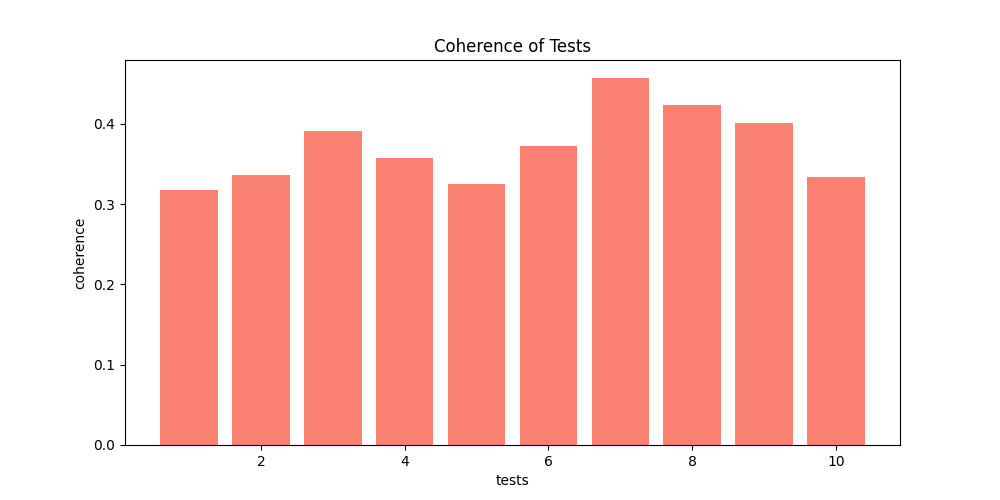
\includegraphics[width=7.5cm]{images/coherence_stopwords}
		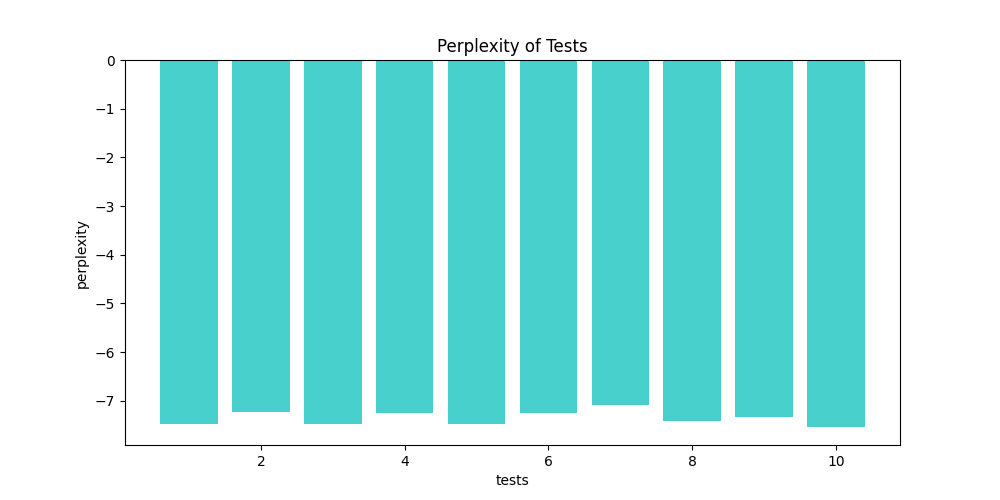
\includegraphics[width=7.5cm]{images/perplexity_stopwords}
	\end{center}

%	\begin{figure}[H]
%		\centering
%		\begin{tabular}{|c|c|c|}
%			\hline \textbf{Test} & \textbf{Perplexity} & \textbf{Coherence}  \\  
%			\hline \textbf{1} & -7.49 & 0.82 \\
%			\hline \textbf{2} & -7.59 & 0.67\\
%			\hline \textbf{3} & -7.82 & 0.70 \\
%			\hline \textbf{4} & -7.46 & 0.79 \\
%			\hline \textbf{5} & -7.25 & 0.70 \\
%			\hline \textbf{6} & -8.05  & 0.57 \\
%			\hline \textbf{7} & -7.21 & 0.84 \\
%			\hline \textbf{8} & -7.76 & 0.63 \\
%			\hline \textbf{9} & -7.99 & 0.64 \\
%			\hline \textbf{10} & -7.56 & 0.81 \\
%			\hline
%		\end{tabular}
%	\end{figure}
	
	The first thing we can notice is that different coherence and perplexity values are obtained in each run, even though we are working with the same corpus and number of topics. 
		
	In the LDA (\textit{Latent Dirichlet Allocation}) model, coherence and perplexity can vary when running the model multiple times with the same set of words. This can be attributed to various factors, such as random initialization of the model, parameter selection, quality of the training corpus, and the amount of available data. Additionally, different implementations of LDA may have variations in how coherence and perplexity are calculated, which can also contribute to differences in results. To address the issue of variability in coherence and perplexity in the LDA model of gensim when running it multiple times with the same set of words we can use a fixed random seed ensuring consistent initializations and obtaining more stable results. 
	
	The average values of perplexity and coherence across tests is approximately -7.62 and 0.72.
	
	\subsection{Topic descriptions obtained with one specific launch}
	
	To further analyze the performance of the model let's look at the topic description obtained with one specific launch, in this case, test 8:
	
	\begin{center}
		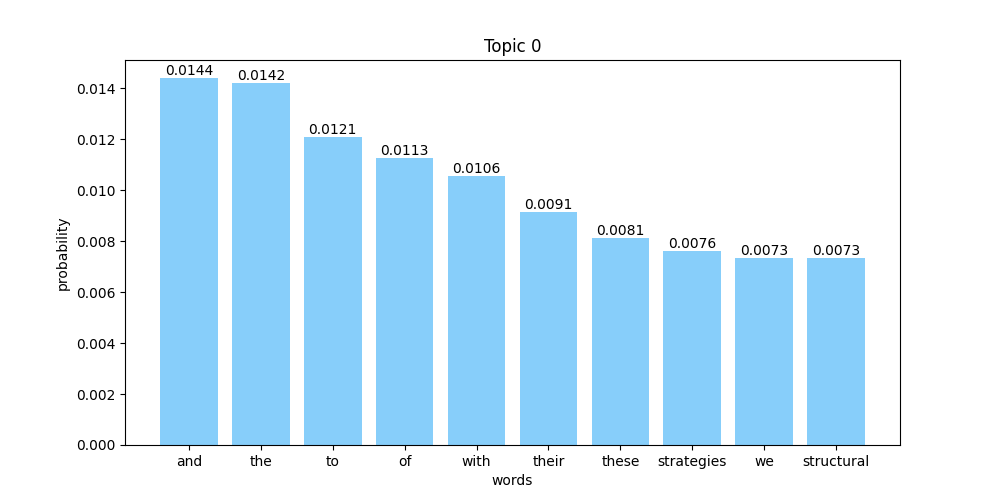
\includegraphics[width=7.5cm]{images/plots/test_8/topic_0.png}
		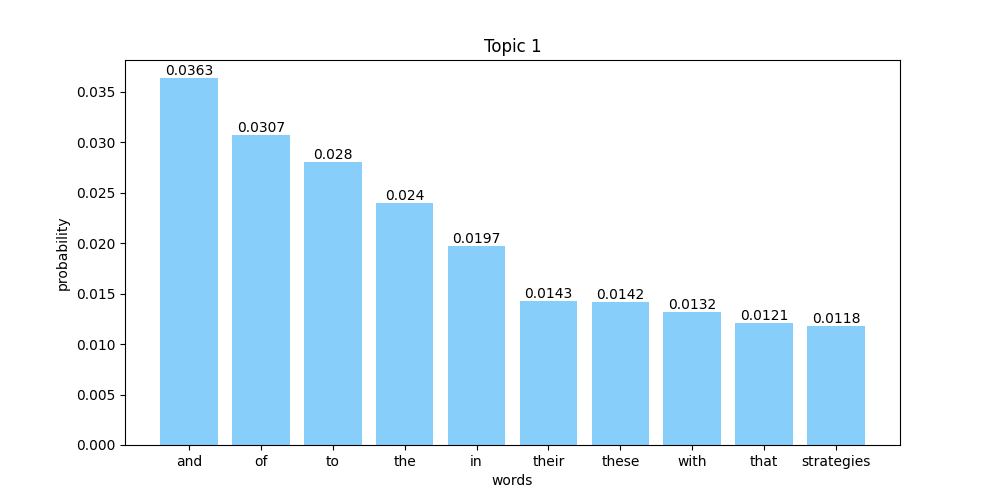
\includegraphics[width=7.5cm]{images/plots/test_8/topic_1.png}
		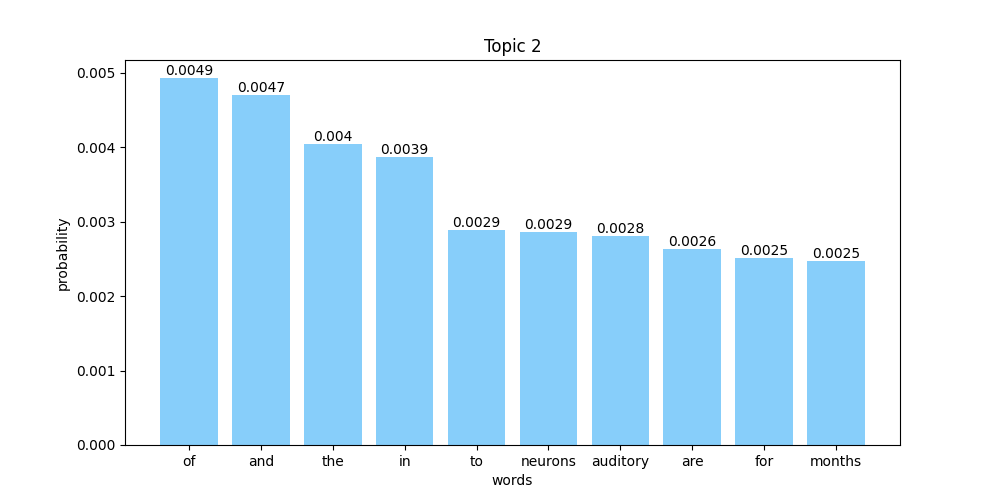
\includegraphics[width=7.5cm]{images/plots/test_8/topic_2.png}
		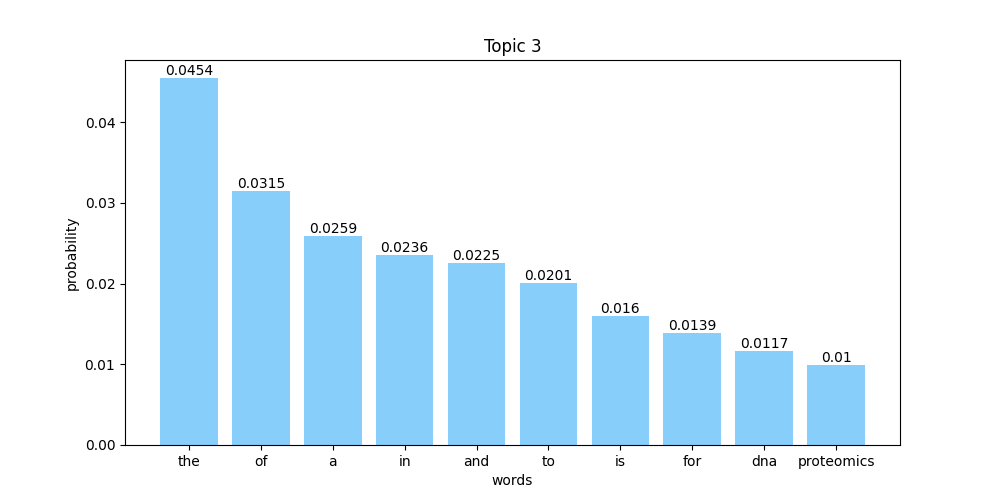
\includegraphics[width=7.5cm]{images/plots/test_8/topic_3.png}
		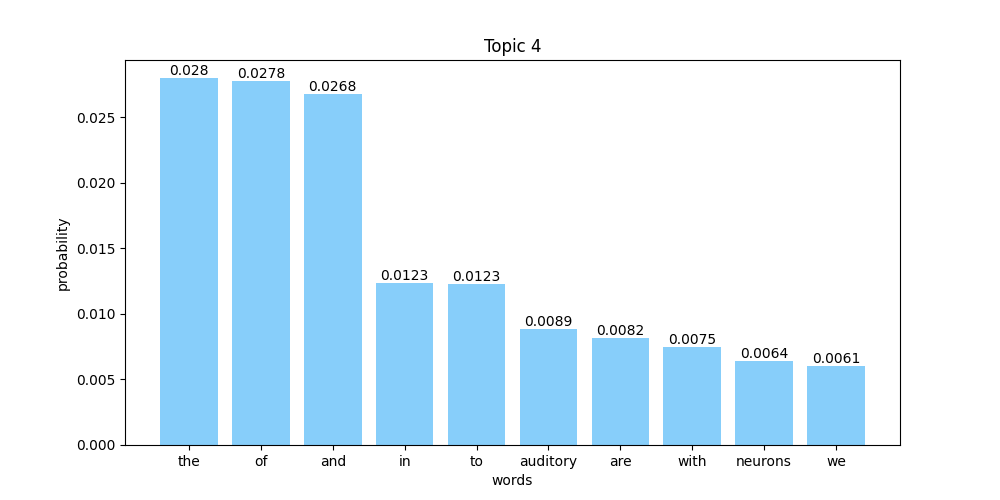
\includegraphics[width=7.5cm]{images/plots/test_8/topic_4.png}
		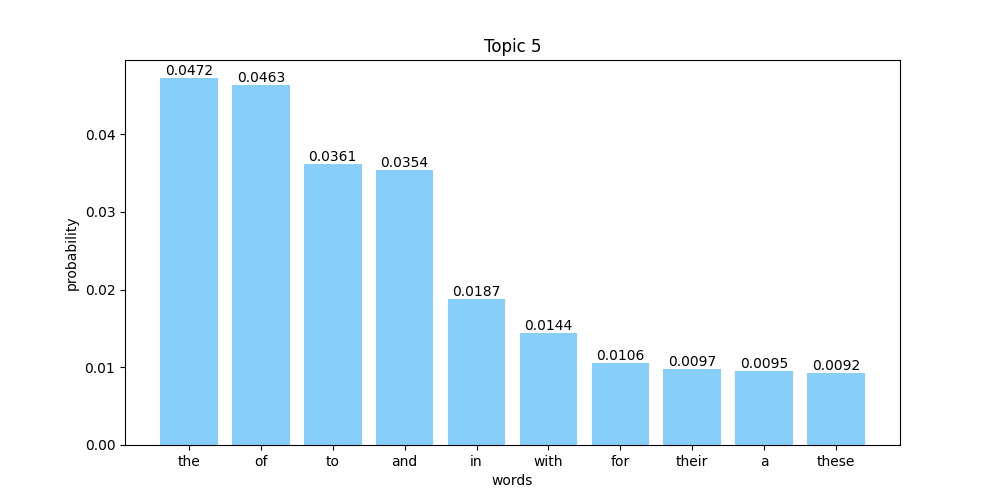
\includegraphics[width=7.5cm]{images/plots/test_8/topic_5.png}
		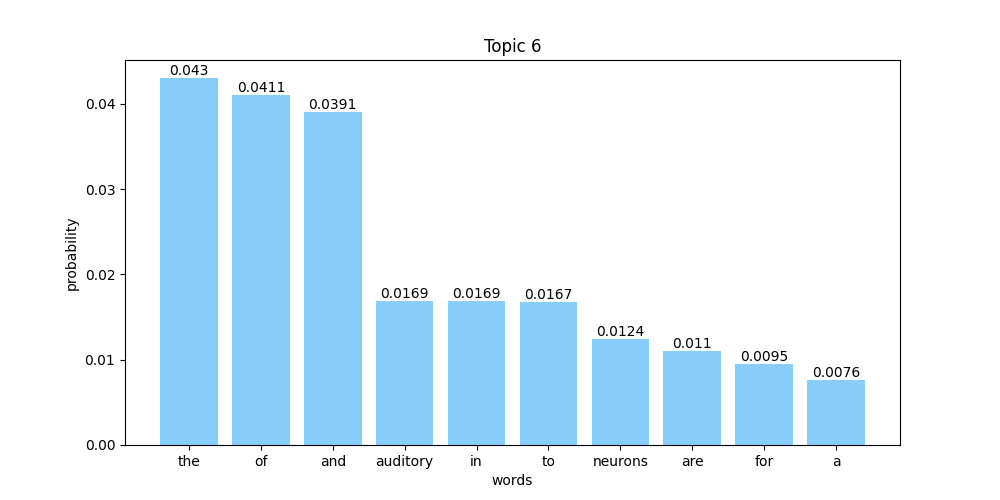
\includegraphics[width=7.5cm]{images/plots/test_8/topic_6.png}
		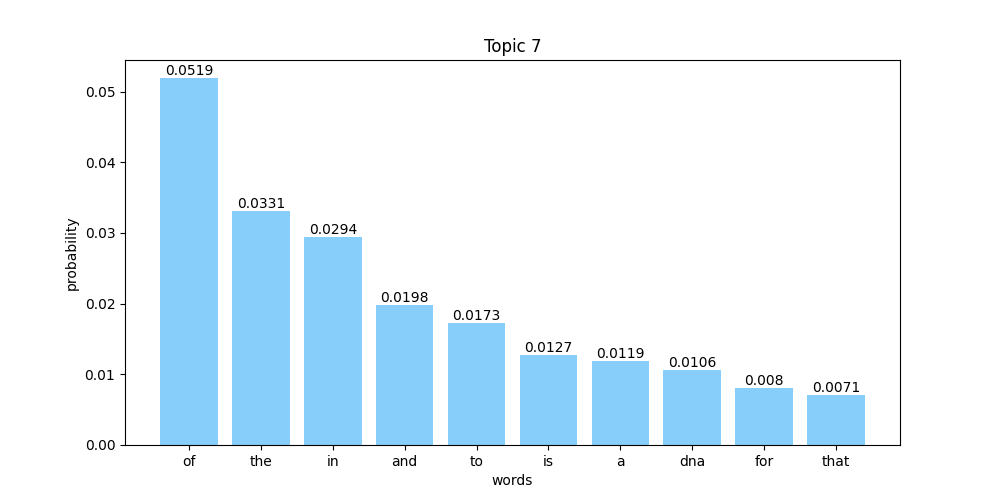
\includegraphics[width=7.5cm]{images/plots/test_8/topic_7.png}
	\end{center}

	A significant issue was observed. The majority of the words that emerged in the topic descriptions were identified as stopwords. 
	
	\textit{Stopwords} are commonly used words in a language that are usually filtered out before or after processing of natural language data. Typically they consist in articles, prepositions, conjunctions, or pronouns. Examples of stopwords in English include "a", "the", "is", "are", and so on. The presence of these stopwords in the topic descriptions is problematic because they appear in almost every document. They are generally uninformative in the context of an LDA model, as they do not contribute to the theme or subject of a topic. The high prevalence of stopwords in the topic descriptions makes it challenging to interpret the topics and understand the underlying themes in the dataset.
	
	In terms of the model's performance metrics, the coherence value is relatively low, 0.37, which is consistent with the observation that the topics are difficult to interpret due to the high presence of stopwords. The perplexity value was -7.26 which does not provide a clear indication of the model's performance. 
	
	\section{Removing stopwords}
	
	The removal of stopwords in the Latent Dirichlet Allocation (LDA) model indeed plays a crucial role in enhancing the quality of the topics generated. By eliminating these common words, which typically do not contribute to the meaning or theme of a topic, the model can focus on the most significant words for topic identification. This not only improves the interpretability of the topics but also reduces the dimensionality of the word space used, making the model more efficient.
	
	A new Python script was created in which the lines of code responsible for removing stopwords from the given set of words in TokenVieuxM.txt were uncommented. This modification is expected to improve the performance of the model. 
	
	\begin{center}
		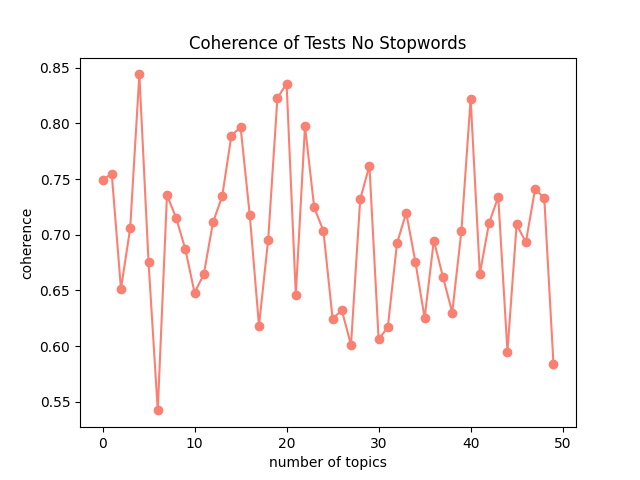
\includegraphics[width=7.5cm]{images/coherence_no_stopwords}
		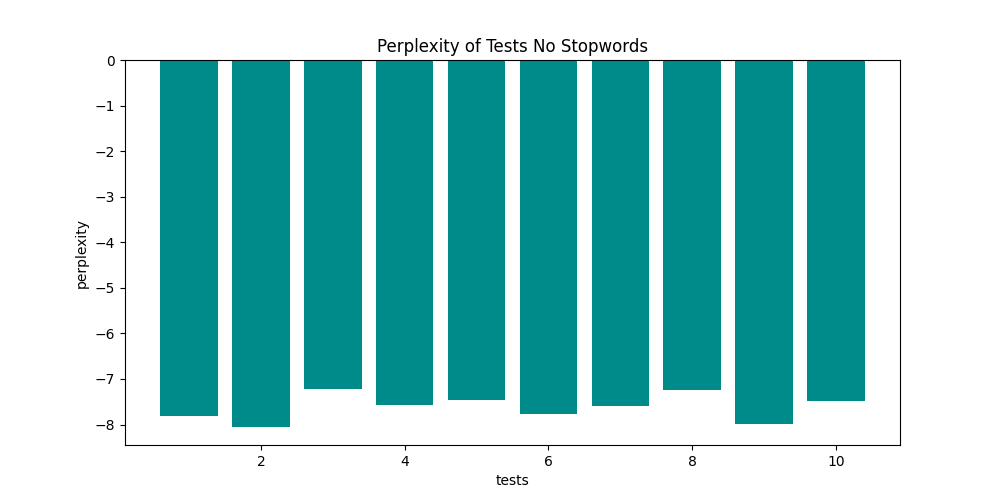
\includegraphics[width=7.5cm]{images/perplexity_no_stopwords}
	\end{center}
	
	\todo{agregar valores promedio de c y p}
	
	\subsection{Topic descriptions obtained with one specific launch and no stopwords}\label{test_8_ns_1}
	
	Once again, let's look at the topic description obtained with one specific launch of test 8:
	
	\begin{center}
		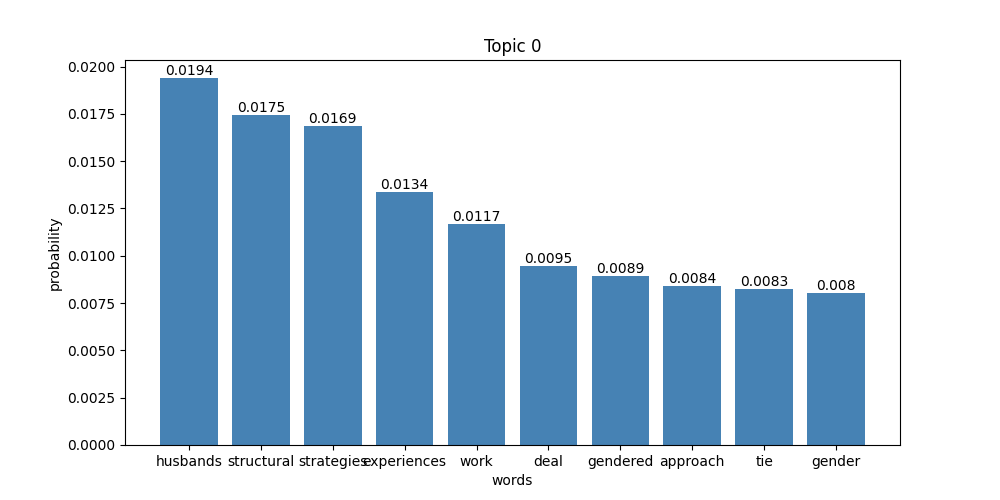
\includegraphics[width=7.5cm]{images/plots/test_8_no_stopwords/topic_0.png}
		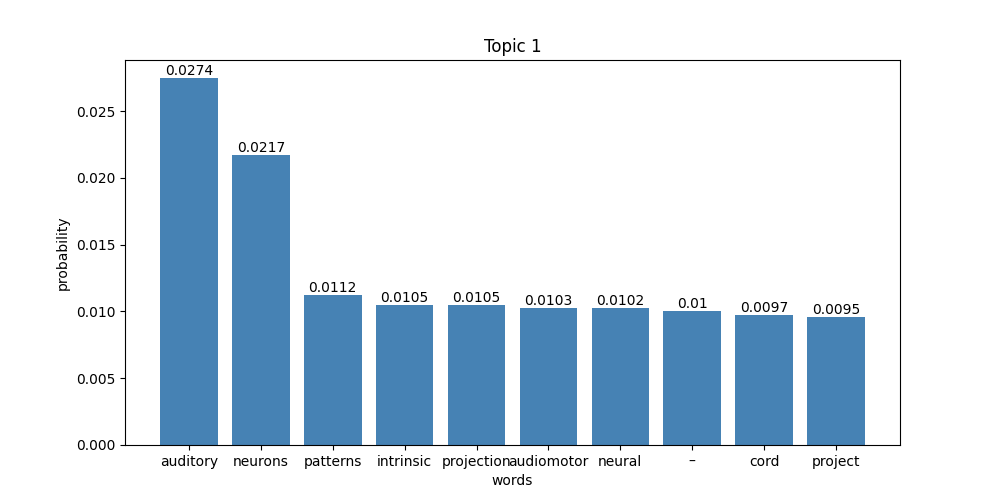
\includegraphics[width=7.5cm]{images/plots/test_8_no_stopwords/topic_1.png}
		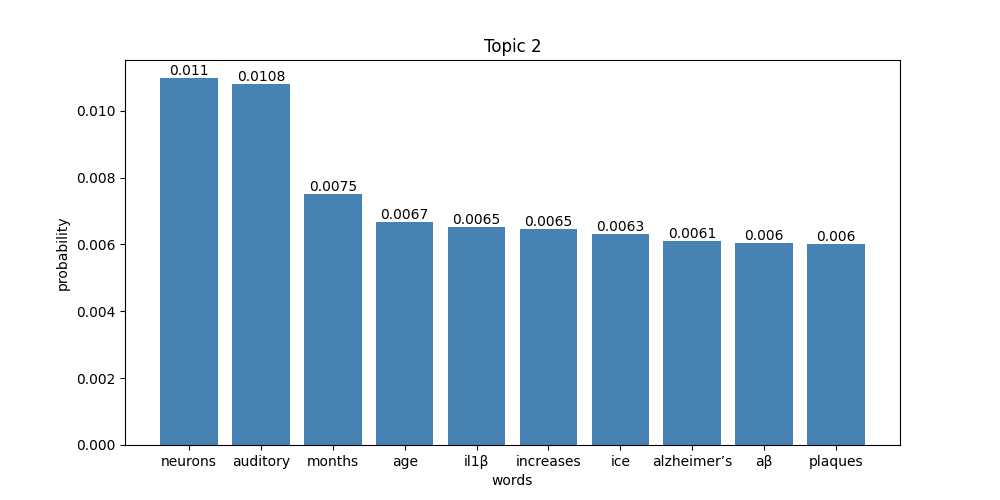
\includegraphics[width=7.5cm]{images/plots/test_8_no_stopwords/topic_2.png}
		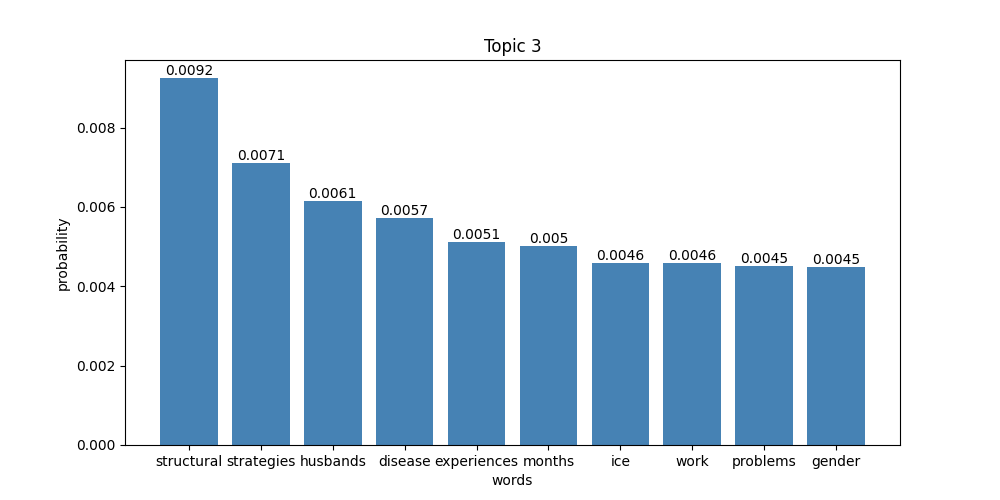
\includegraphics[width=7.5cm]{images/plots/test_8_no_stopwords/topic_3.png}\
		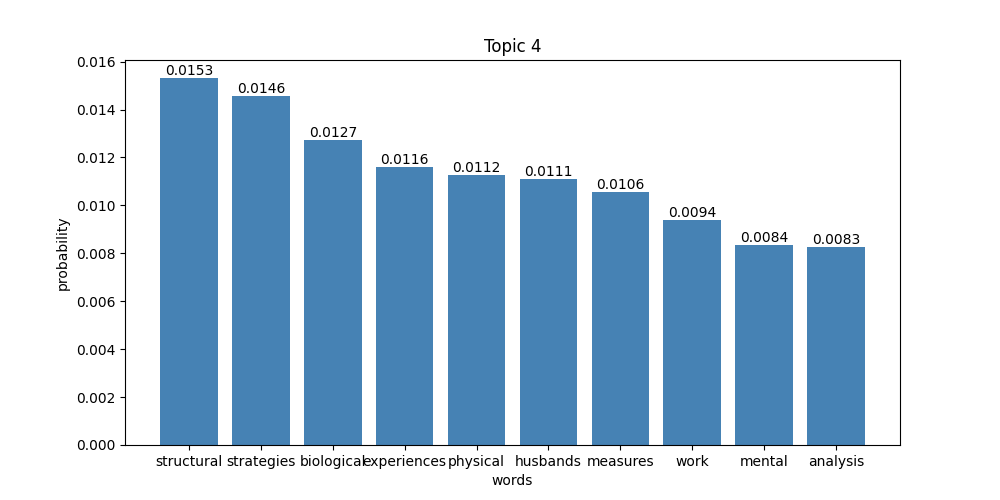
\includegraphics[width=7.5cm]{images/plots/test_8_no_stopwords/topic_4.png}
		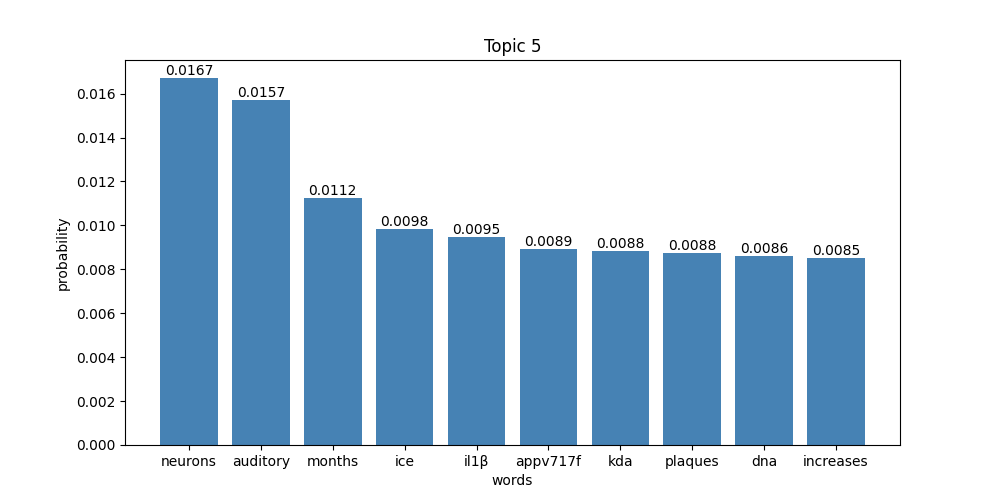
\includegraphics[width=7.5cm]{images/plots/test_8_no_stopwords/topic_5.png}
		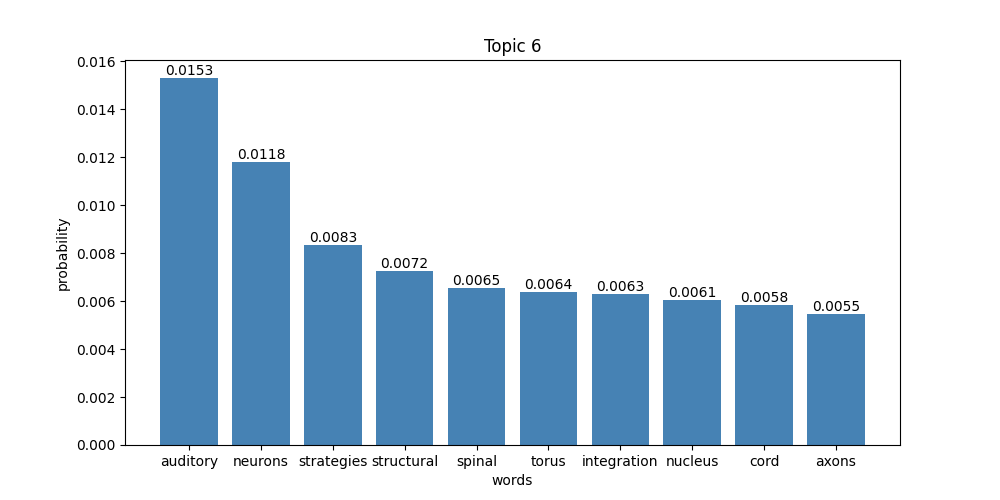
\includegraphics[width=7.5cm]{images/plots/test_8_no_stopwords/topic_6.png}
		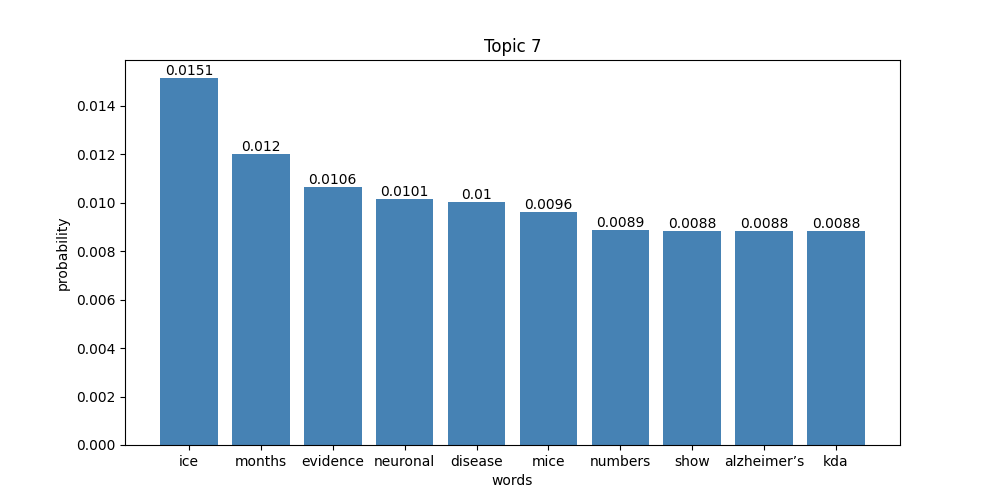
\includegraphics[width=7.5cm]{images/plots/test_8_no_stopwords/topic_7.png}
	\end{center}

	La perplexity es -7.764361092424768 y la coherencia  0.6284575950301475.
	
	\section{Comparing results}
	
	\todo{2.c hay que comparar los resultados con el test sin remover stopwords y ver la relaci\'on entre coherencia y perplexity}
	
	\section{Optimal number of topics for the document collection TokenVieuxM.txt}
	
	\todo{2.d Escribir cual ser\'ia el n\'umero \'optimo de t\'opicos y por qu\'e}
	
	\begin{center}
		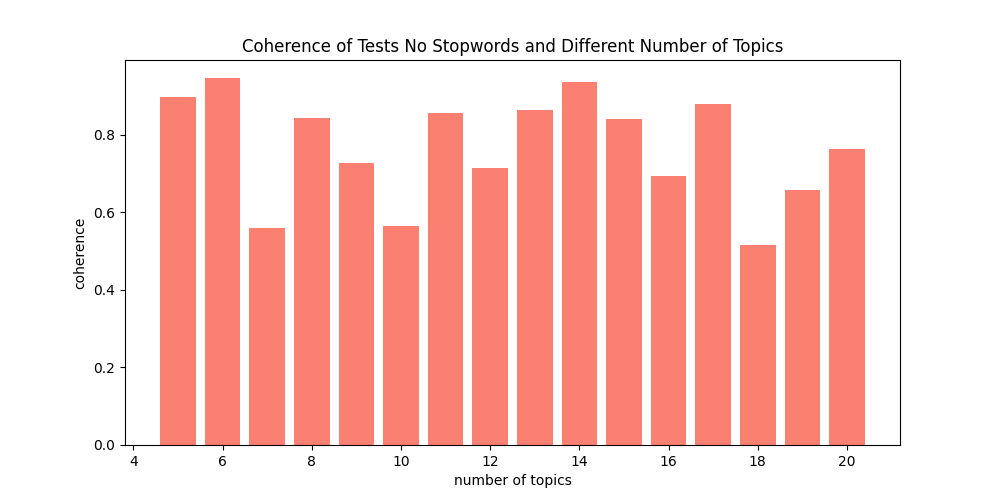
\includegraphics[width=7.5cm]{images/coherence_no_stopwords_diff_n_topics}
		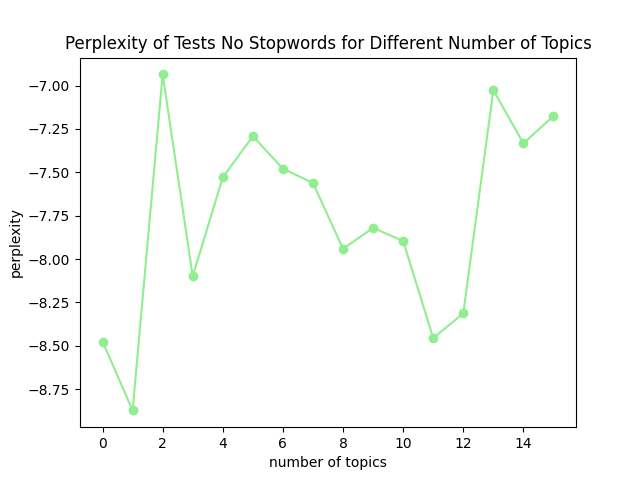
\includegraphics[width=7.5cm]{images/perplexity_no_stopwords_diff_n_topics}
	\end{center}

	El n\'umero \'optimo de t\'opicos de acurdo a los valores de coherencias deber\'ia ser 6.
	
	\section{Changing the dataset}
	
	\begin{center}
		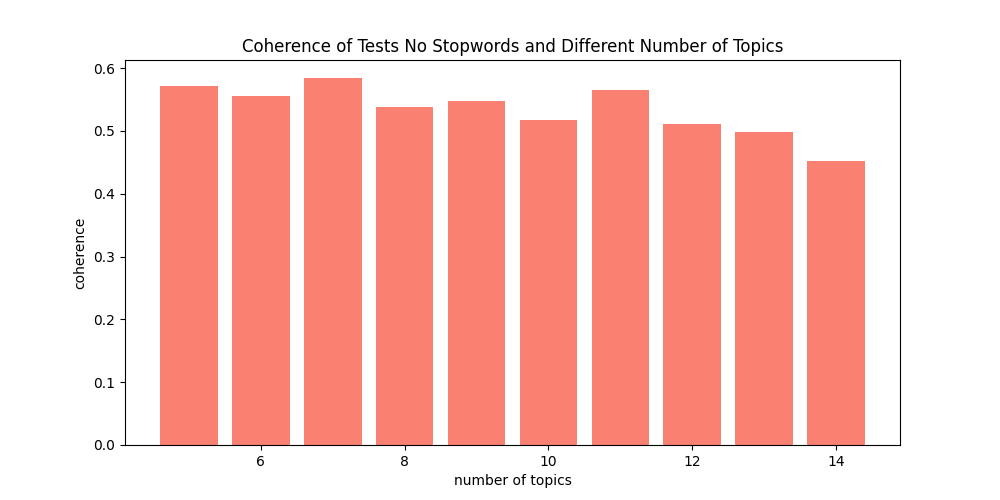
\includegraphics[width=7.5cm]{images/coherence_no_stopwords_2}
		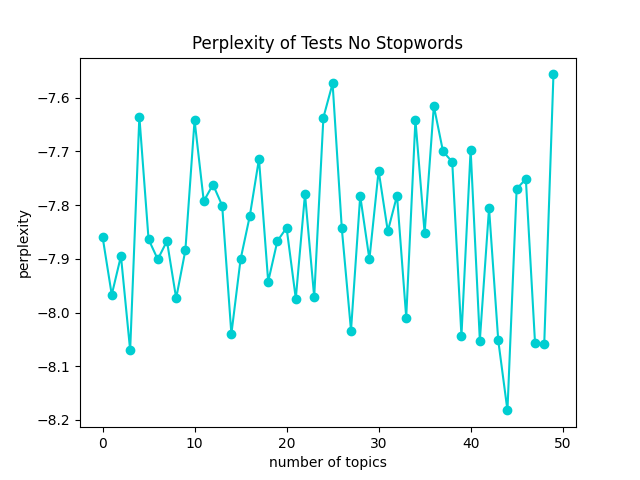
\includegraphics[width=7.5cm]{images/perplexity_no_stopwords_2}
	\end{center}
	
	\subsection{Topic descriptions obtained with one specific launch and no stopwords}
	
	\todo{2.e Comparar los resultados de este dataset con el \ref{test_8_ns_1} y llegar a conclusiones.}
	\begin{center}
		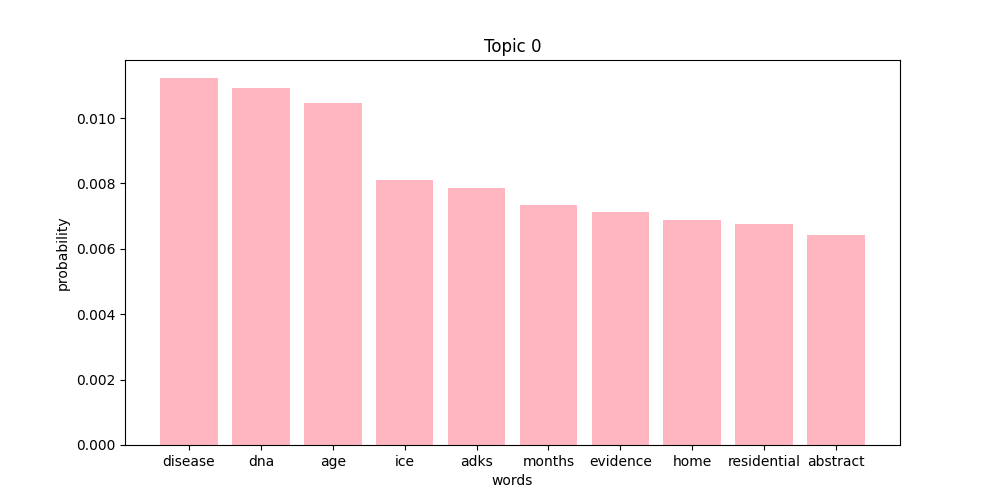
\includegraphics[width=7.5cm]{images/plots/test_8_no_stopwords_dataset_2/topic_0.png}
		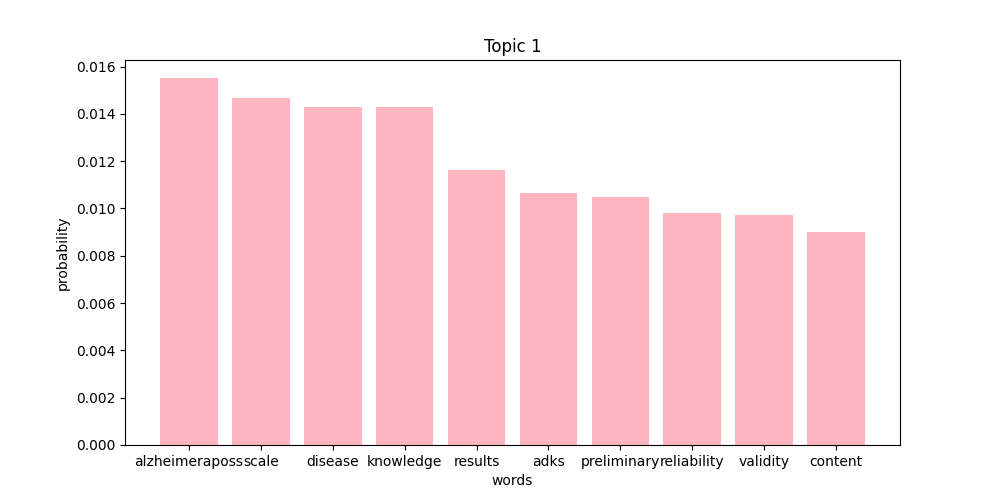
\includegraphics[width=7.5cm]{images/plots/test_8_no_stopwords_dataset_2/topic_1.png}
		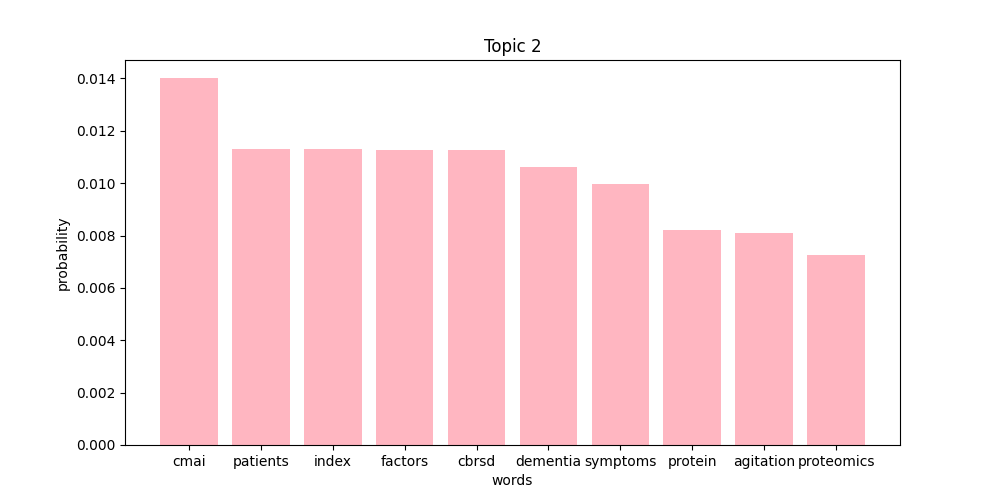
\includegraphics[width=7.5cm]{images/plots/test_8_no_stopwords_dataset_2/topic_2.png}
		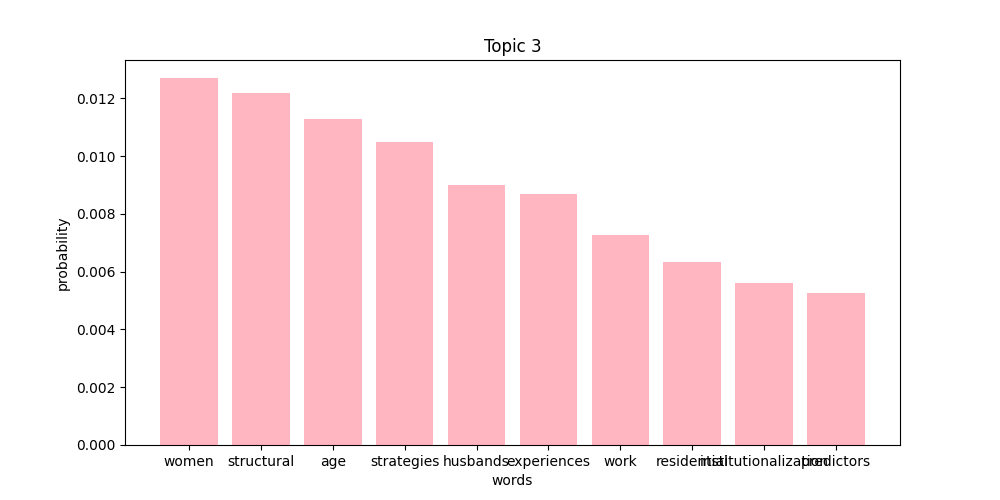
\includegraphics[width=7.5cm]{images/plots/test_8_no_stopwords_dataset_2/topic_3.png}\
		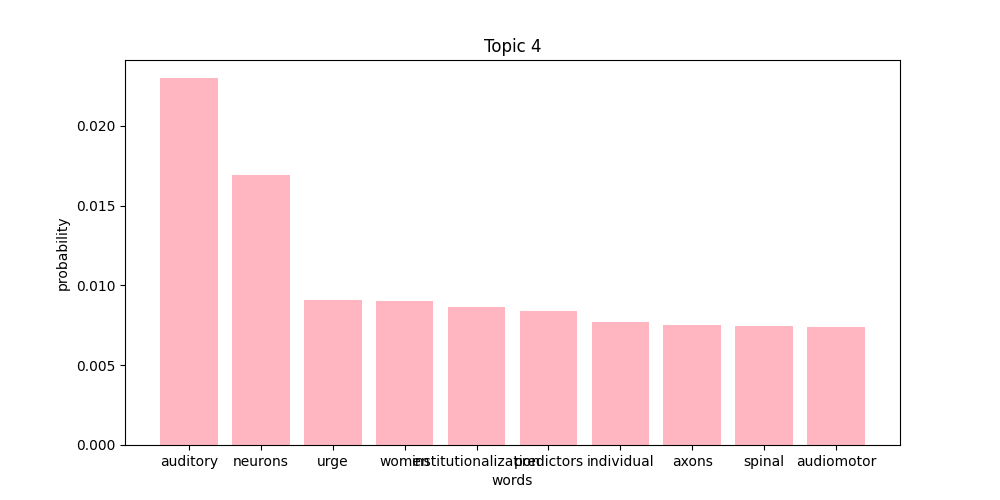
\includegraphics[width=7.5cm]{images/plots/test_8_no_stopwords_dataset_2/topic_4.png}
		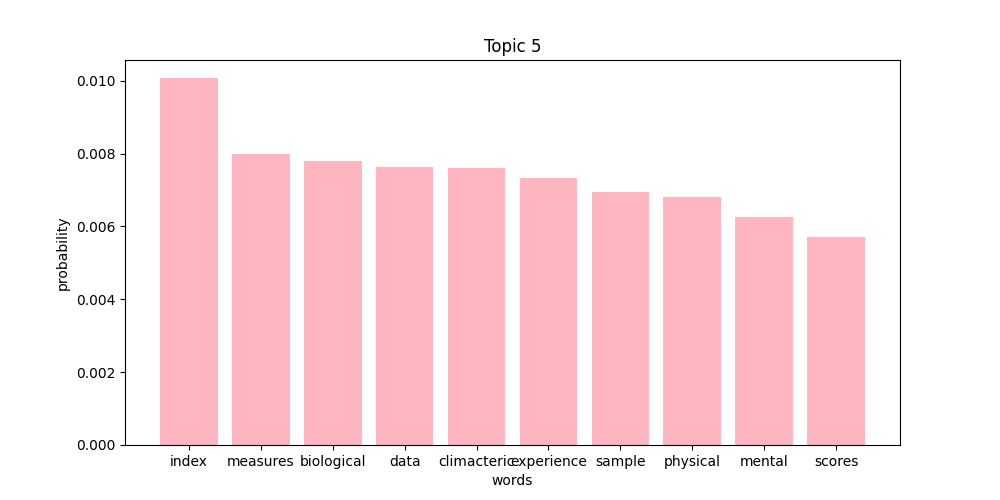
\includegraphics[width=7.5cm]{images/plots/test_8_no_stopwords_dataset_2/topic_5.png}
		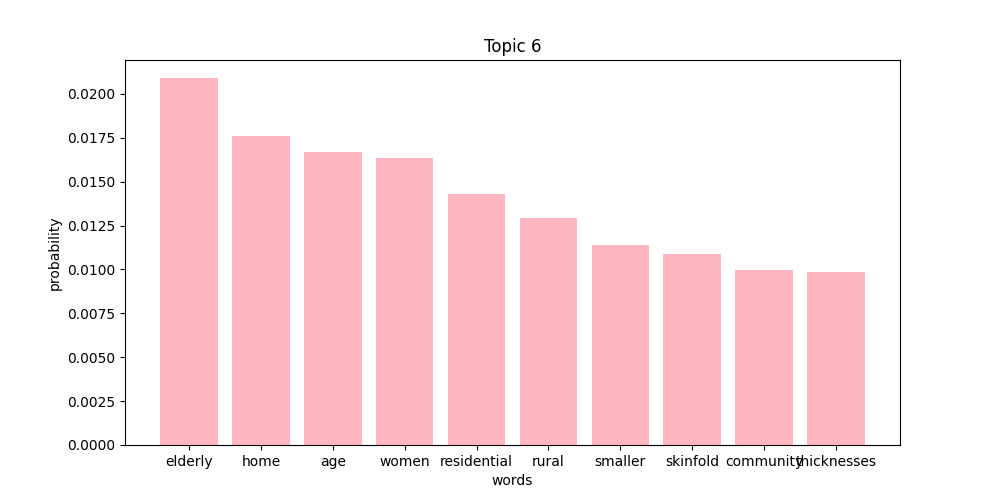
\includegraphics[width=7.5cm]{images/plots/test_8_no_stopwords_dataset_2/topic_6.png}
		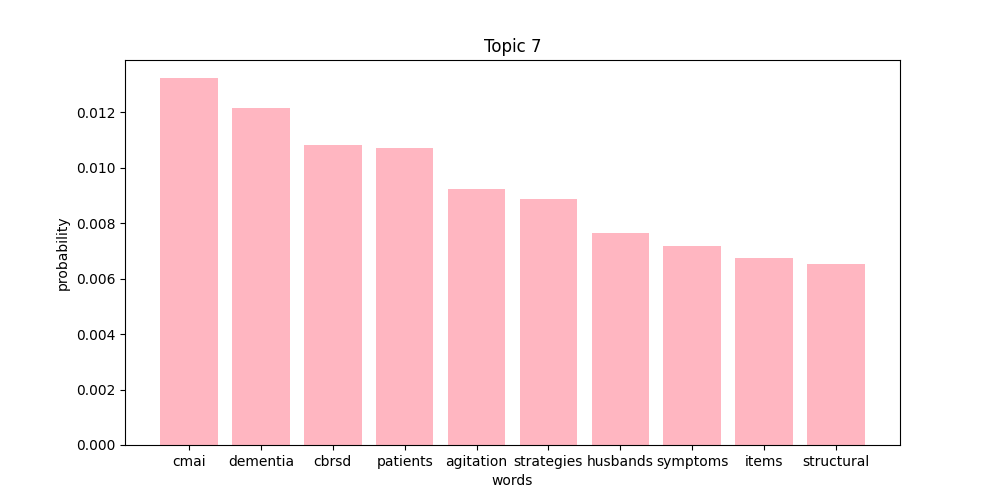
\includegraphics[width=7.5cm]{images/plots/test_8_no_stopwords_dataset_2/topic_7.png}	
	\end{center}

	\subsection{Optimal number of topics for the document collection TokenVieuxN.txt}
	\todo{2.f Analizar cu\'al es el n\'umero de t\'opicos \'optimo y justificar}
	\begin{center}
		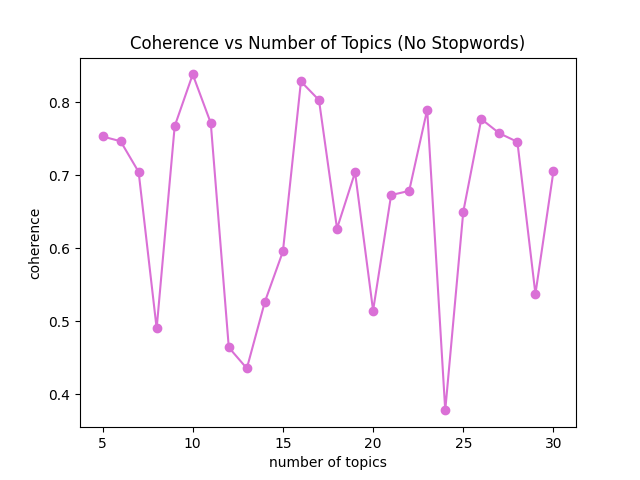
\includegraphics[width=7.5cm]{images/coherence_no_stopwords_diff_n_topics_2}
		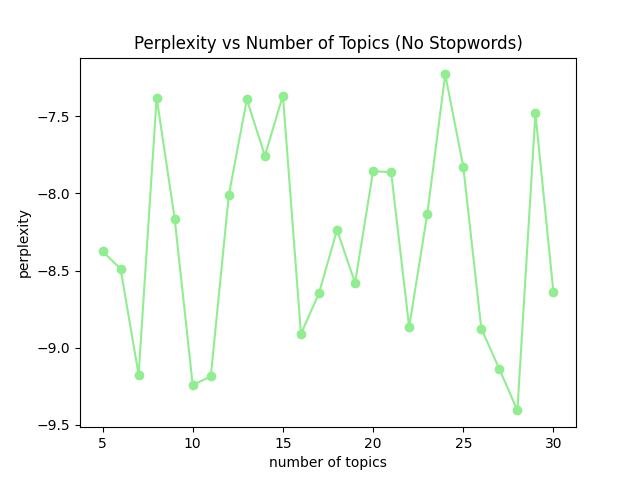
\includegraphics[width=7.5cm]{images/perplexity_no_stopwords_diff_n_topics_2}
	\end{center}
	
	\section{Most typical documents for topics}
	\todo{Ver como utilizar el m\'etodo}
	Para identificar el documento más típico en cada tópico utilizando LDA de Gensim en Python, puedes utilizar el método get\_document\_topics proporcionado por la clase LdaModel. Este método devuelve una lista de tuplas que contienen el ID del tópico y la probabilidad de ese tópico para cada documento.
	
	
	\section{Code modifications, tests and plots}
	
	The Python program used for this analysis was divided into three main functions: `read()`, `parse()`, and `lda()`.
	
	The `read()` function is responsible for reading the indicated dataset. The `parse()` function processes the read dataset, removing unnecessary symbols and preparing the data for the LDA model. The `lda()` function initializes an LDA model from the Gensim module, to which the parsed dataset and the number of topics to be generated are passed. This function also calculates the coherence and perplexity of the model.
	
	
	\begin{thebibliography}
		a
		\bibitem{introduction} Cormen, Thomas H. y otros. \emph{Introduction to Algorithms}. 
		The MIT Press.
		4ta Edici\'on.		
		Cambridge, Massachusetts.
		2022.
		\todo{Actualizar referencias}
	\end{thebibliography}
\end{document}


